% !TeX root = ../main.tex
% Add the above to each chapter to make compiling the PDF easier in some editors.

\chapter{Related Works}\label{chapter:related_works}
In this chapter, works from the literature are presented, which tackle problems related to the presented PHM task in this thesis. In section \ref{sec:traditional_approaches}, traditional PHM approaches for BSDs are discussed, which do not apply any domain adaptation. In chapter \ref{sec:domain_adaption_approach}, deep learning-based domain adaptation approaches are introduced which perform health condition monitoring for BSDs and rolling bearings. In section \ref{sec:domain_adaption_CV}, an advanced domain adaptation approach from the computer vision community is presented. 

\section{Traditional Approaches for Prognostic and Health Management}\label{sec:traditional_approaches}

Traditionally, model-based and data-driven models were used for PHM. Model-based methods predict the health condition based on physical models describing the underlying degradation mechanisms. Uncertainties in the processes of the machine and noise make developing accurate physical models challenging. Often, the identification of all model parameters is complex and requires extensive experiments. Data-driven methods learn a mapping relationship between the health condition status and monitoring data. Such methods do not use physical information about the degradation process. The performance of data-driven approaches highly depends on the quality and amount of the training data. Since the data-driven models are optimized to perform well in the working conditions represented in the training data, these approaches might lack generality. Both model-based and data-driven approaches suffer from different limitations \cite{DENG2020}. The following presents, traditional data-driven and model-based PHM systems for monitoring the health condition of BSDs are presented.

\subsection{Model-Based Approach: Monitoring of Defect Frequencies Calculated from Rolling Bearings and Transferred to Ball Screw Feed Drives}
Lee et al. \cite{Lee2015} proposed a diagnosis system for estimating the flaking degradation of BSD screw shafts. By filtering the machine signals for previously calculated characteristic defect frequencies, the severity and location of the degradation were predicted. Lee et al. developed a testbed containing one BSD and linear motion guides. An accelerometer was mounted on the BSD nut. Holes with a diameter of 3 mm were punched in the BSD screw shaft to simulate the degradation. The continuous fatigue process was modeled by increasing the number of holes in the BSD screw shaft. Machine signals show the corresponding defect pattern if the steel balls pass a hole in the screw shaft surface. Therefore, vibration signals contain expressive information about the degradation status of BSDs. The motor was actuated with a constant velocity while the data was recorded. Harris and McCool \cite{Harris1996} proposed a method to estimate the characteristic defect frequencies of rolling bearings. Lee et al. \cite{Lee2015} extended that method to make it applicable for BSDs. The BSD screw shafts were considered as inner rings and the BSD nuts as outer rings of the rolling bearings. From the BSD construction details and relative speeds, defect frequencies were calculated. The ball pass frequencies of the shaft (BPFS), the ball pass frequencies of the nut (BPFN) and the ball spin frequency (BSF) were considered as defect frequency: 
\begin{equation}
    BPFS = \frac{1}{120}zn(1+\frac{D_{w}}{d_{m}}cos\alpha),
    \label{eq:defect_frequency}
\end{equation}
\begin{equation}
    BPFN = \frac{1}{120}zn(1-\frac{D_{w}}{d_{m}}cos\alpha),
\end{equation}
\begin{equation}
    BSF = \frac{1}{120}n\frac{d_{m}}{D_{w}} (1-\frac{D_{w}}{d_{m}}cos\alpha)(1+\frac{D_{w}}{d_{m}}cos\alpha) ,
\end{equation}
where $\alpha$ is the contact angle between the ball, nuts and screw shaft, $d_{m}$ is the pitch diameter of the balls, $D_{w}$ is the diameter of a single ball, the rotational speed of the BSD screw shaft is defined by $n$ and $z$ is the number of steel balls. A more detailed visualization of the bearing parameters is shown in fig. \ref{fig:defect_frequency_calc}. 

\begin{figure}[H]
  \centering
  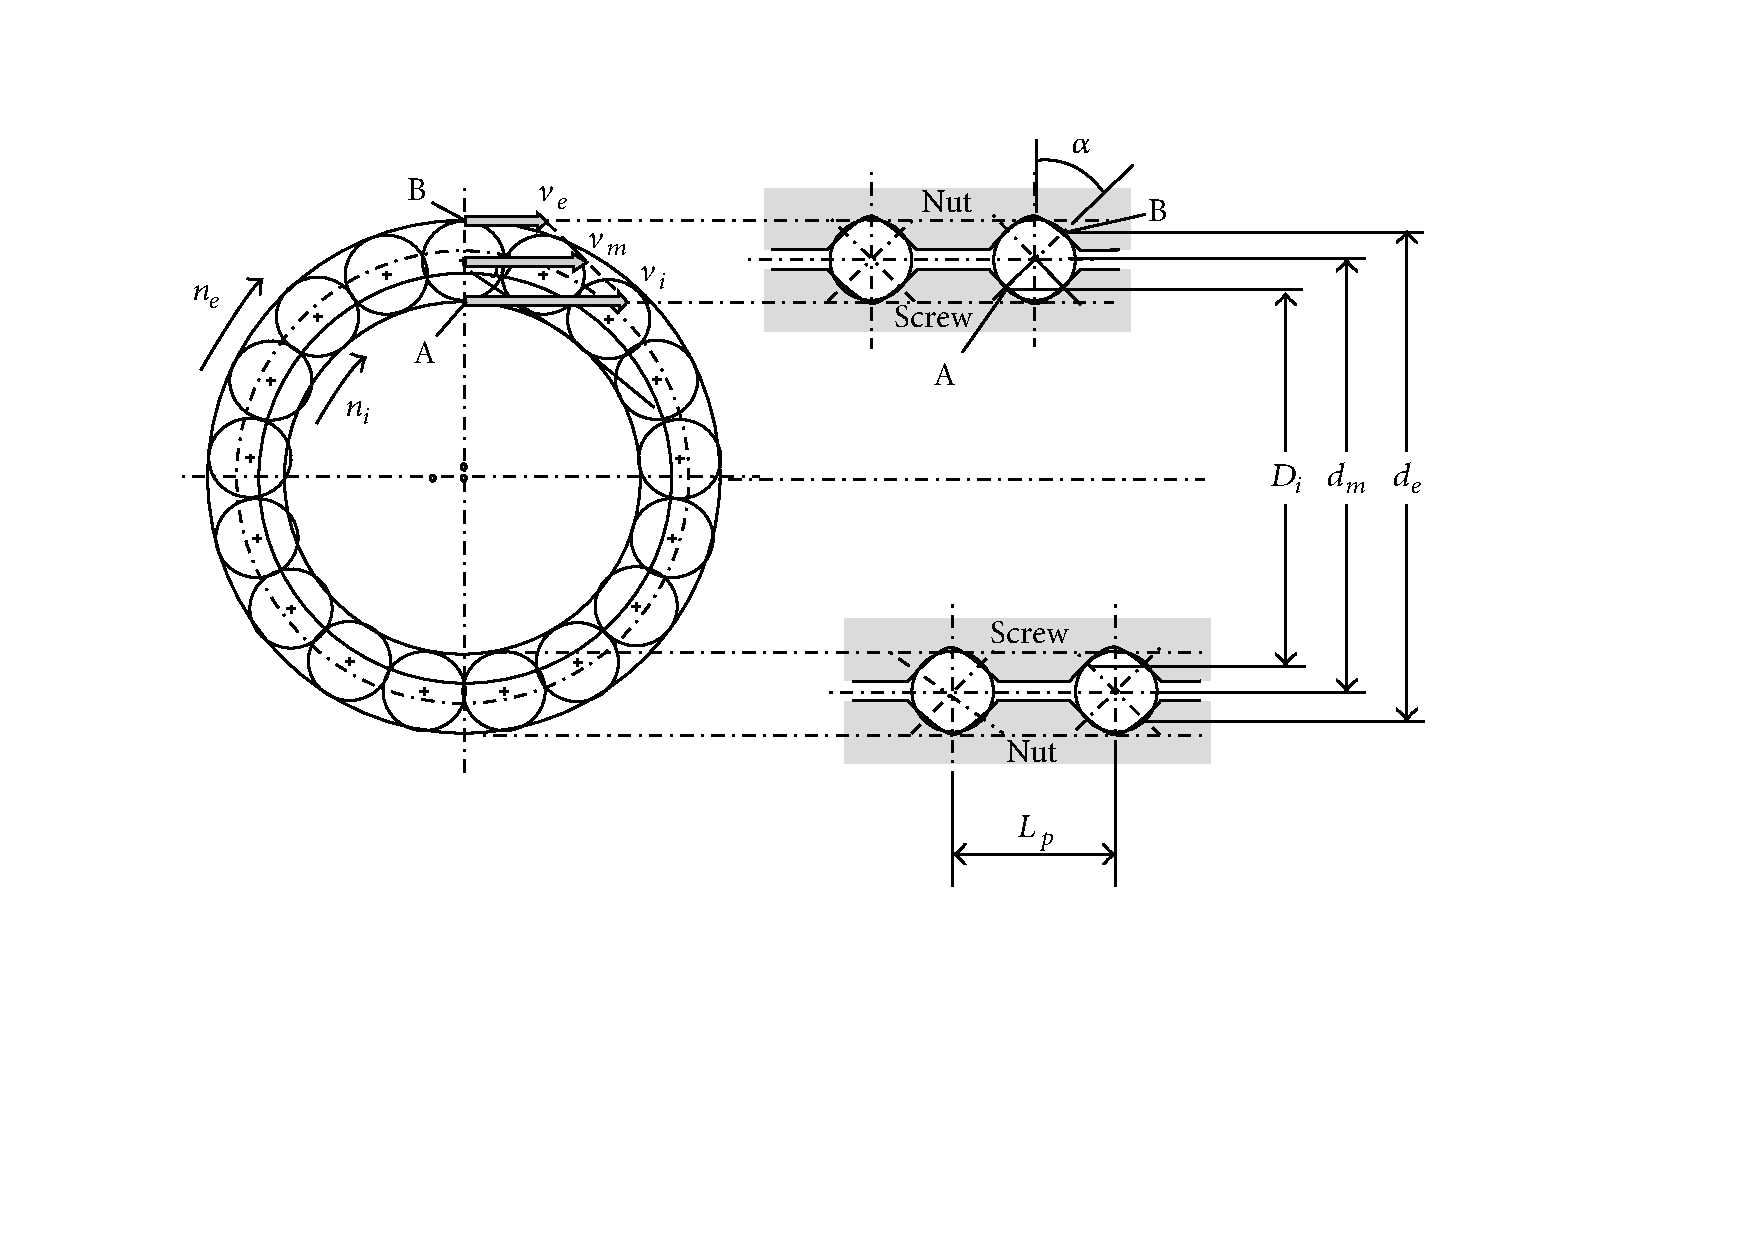
\includegraphics[width=.6\textwidth]{models_state_of_the_art/defect_frequency_calc.pdf}
  \caption{Visualization of the rolling bearing parameters required for the calculation of the defect frequencies \cite{Lee2015}}
  \label{fig:defect_frequency_calc}
\end{figure}

The derived frequencies above are valid for rolling bearings. To apply those to BSDs $z$ and $d_{m}$ need to be replaced by the effective number of steel balls $z^{'}$ and effective pitch parameter $d_{m}^{'}$, which are defined as follows:

\begin{equation} \label{eq:transfer_RollingBearing_BSD}
    d_{m}^{'} = (L_{p}^{2}+(\pi D_{b})^{2})^{\frac{1}{2}},
\end{equation}
\begin{equation}
    z^{'} = \frac{d_{m}^{'}}{D_{w}}.
\end{equation}

The relation between the regular and effective parameters and other required parameters for equation \ref{eq:transfer_RollingBearing_BSD} are visualized in fig. \ref{fig:defect_frequency_transfer}. 

\begin{figure}[H]
  \centering
  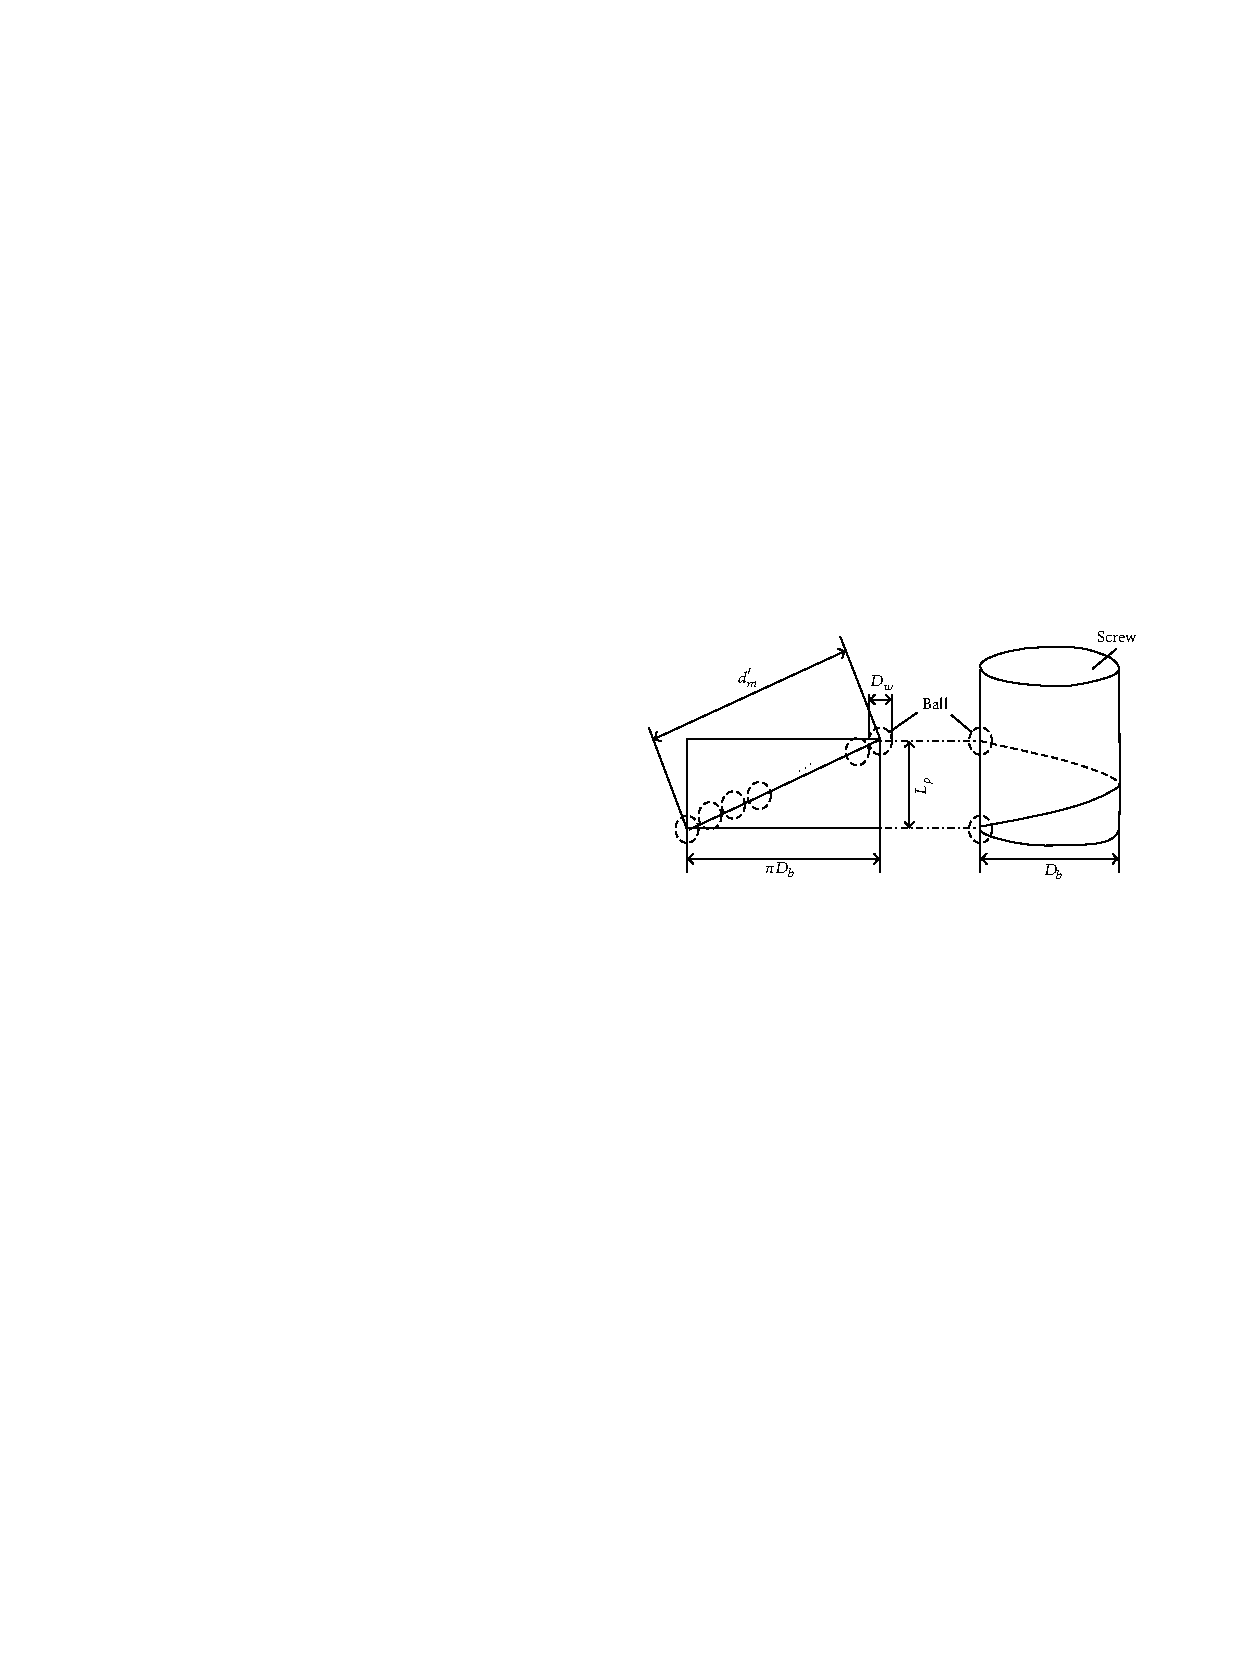
\includegraphics[width=.7\textwidth]{models_state_of_the_art/defect_frequency_transfer.pdf}
  \caption{Relationship between the regular and effective parameters required for transferring the calculated defect frequencies to the BSDs \cite{Lee2015}}
  \label{fig:defect_frequency_transfer}
\end{figure}

The BPFS frequency was identified as the most expressive and reliable for supervising the health condition of BSDs. To calculate the BPFS for ball screw feed drives, the equation \ref{eq:defect_frequency} must be combined with the effective pitch parameter $d_{m}^{'}$ and the effective number of steel balls $z^{'}$. During testing, the wavelet transform (Daubechies Wavelet (db14) function) was used to transform the machine signals in the two-dimensional time-frequency domain. By supervising the magnitude of the calculated defect frequency in the machine signal's time-frequency domain, the BSD's degradation status was monitored. An alarm was triggered when the degradation was not acceptable anymore. The time-related information was an indicator of the defect location. The frequency-related information provided information about the degradation status of the BSD. The proposed approach during testing is visualized in fig. \ref{fig:defect_frequency_model}. 


\begin{figure}[H]
  \centering
  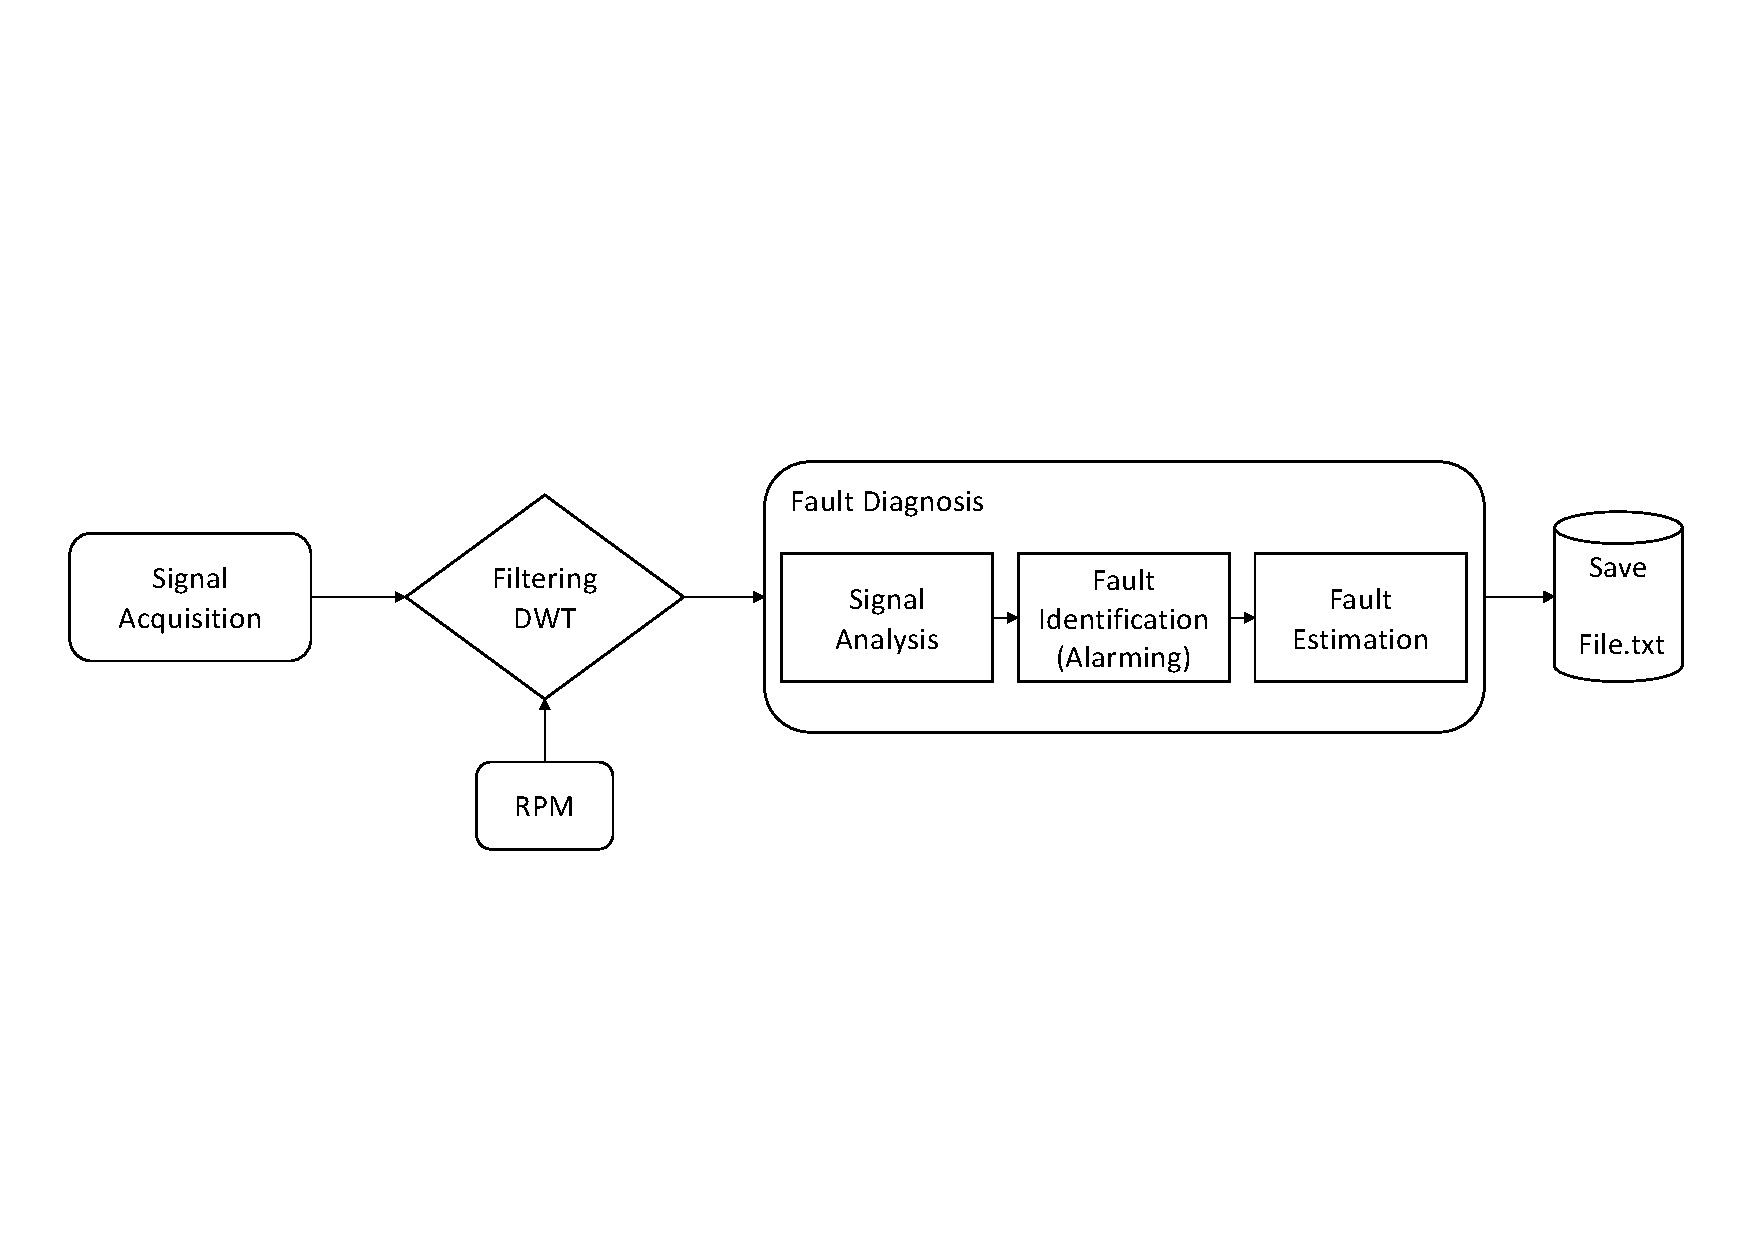
\includegraphics[width=.95\textwidth]{models_state_of_the_art/defect_frequency_model.pdf}
  \caption{Failure diagnosis system during tetsing based on \cite{Lee2015}}
  \label{fig:defect_frequency_model}
\end{figure}

\subsubsection{Conclusion}
Lee et al. \cite{Lee2015} assumed that defects and degradation are mainly subjected to rolling friction. Such simplified assumptions are often made when developing model-based PHM systems. In reality, the balls in the BSDs are rotating, revolving, and sliding \cite{Lee2015}. These highly complex processes make accurate degradation modeling, which is essential to achieving a good PHM performance, more challenging. In data-driven PHM systems, the correlation between the machine data and degradation patterns can be learned flexibly. The PHM system can be adapted to predict different degradation patterns and extents by picking expressive signals and defining appropriate health condition classes. Lee et al. \cite{Lee2015} had to stick to the defect frequencies developed by Harris et al. \cite{Harris1996}, which are limited to the flaking-related degradation of BSDs. Adapting the diagnosis system to monitor other degradation types is nearly impossible. Furthermore, different operational conditions of the machine might influence the characteristic defect frequencies. When comparing the frequencies extracted from machine signals with the calculated defect frequencies, Lee et al. observed other distinct frequencies coming from major electrical noise. The proposed method was only tested on a simplified BSD testbed. When applying the approach to real-world machines, vibrations from other components could contaminate the recorded signal. Distinguishing the characteristic frequencies from different components becomes even more challenging in such scenarios. Apart from that, the accelerometer was mounted on the BSD nut, recording the BSD vibration signals. The BSD nut is a highly fault-critical but also a very impractical sensor location for real-world use \cite{Pandhare2021}. It is questionable how this method would work with vibration signals recorded from less fault-critical sensor locations. Finding all parameters to calculate the defect frequencies may require a lot of measuring and testing effort. Often these parameters are assumed to be constant throughout the lifetime of the BSDs. For example, the rolling diameter will be reduced throughout the lifetime of the rolling bearings. Nevertheless, this parameter was used as a constant parameter in the calculation of the BSD's defect frequencies. Only structural differences were considered when transferring the calculated defect frequencies from the rolling bearing to the BSD. The linear movement of the BSDs was completely ignored, representing a fundamental functional difference between rolling bearings and BSDs. The degradation process was simulated by punching holes with a diameter of 3 mm on the grooves of the BSD screw shaft. The ongoing degradation was simulated solely by increasing the number of holes. The variations in the dimension of these holes were not considered.

\subsection{Model-Based Approach: Ball Screw Feed Drive Preload Estimation Based on a Discrete Dynamic Model}
Nguyen et al. \cite{NGUYEN2019} applied a simplified discrete dynamic model (see fig. \ref{fig:Nguyen_discrete_dynamic_model}) to investigate the relation between the preload variations and the dynamic characteristics of BSDs.

\begin{figure}[H]
  \centering
  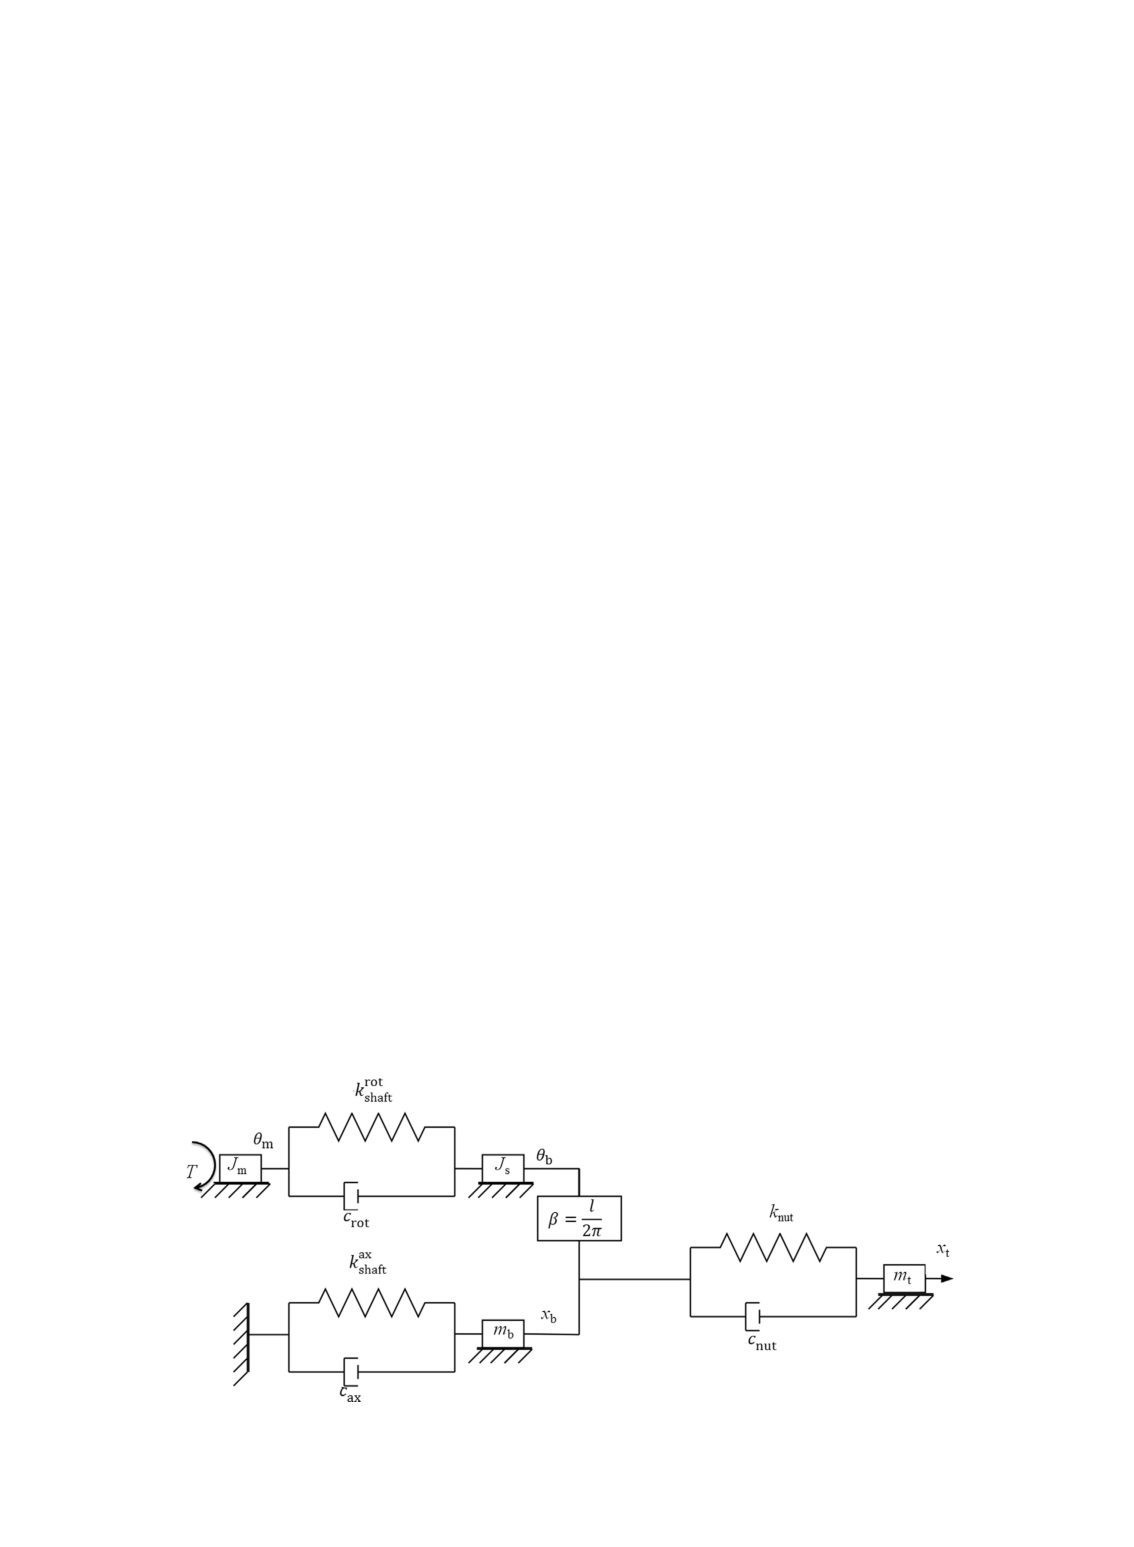
\includegraphics[width=1\textwidth]{models_state_of_the_art/Nguyen_discrete_dynamic_model.pdf}
  \caption{Discrete dynamic model \cite{NGUYEN2019}}
  \label{fig:Nguyen_discrete_dynamic_model}
\end{figure}

According to the discrete dynamic model, the preload variations of BSDs correlate with the screw nut stiffness:

\begin{equation}
    k_{nut}=0.8K(\frac{P}{0.1C_{a}})^{\frac{1}{3}},
\end{equation}

where $P$ is the BSD preload, $C_{a}$ is the BSD screw dynamic load, $K$ is the BSD nut stiffness according to the manufacturer and $k_{nut}$ is the actual BSD nut stiffness. The formula is valid if the BSD preload is less than 10\% of the BSD dynamic load. The axial and rotational stiffness of the BSD screw shaft is determined by the configuration parameters and the working table displacement:
\begin{equation}
    k_{shaft}^{ax}=\frac{EA}{x_{t}}=\frac{\pi}{4x_{t}}d_{minor}^{2}E,
\end{equation}
\begin{equation}
    k_{shaft}^{rot}=\frac{\pi}{32L}d_{minor}^{4}G,
\end{equation}
 where $A$ is the cross sectional area of the BSD screw shaft, $E$ the Young’s modulus, $d_{minor}$ the screw diameter, $G$ the shear modulus, $L$ the screw shaft length and $x_{t}$ the working table displacement. The total axial stiffness of the BSD is composed of the stiffness of the screw shaft, supporting bearing, screw nut, and bracket:
 \begin{equation}
    \frac{1}{k_{ax}}=\frac{1}{k_{shaft}^{ax}}+\frac{1}{k_{bearing}^{ax}}+\frac{1}{k_{nut}^{ax}}+\frac{1}{k_{bracket}^{ax}}+\frac{1}{\frac{k_{shaft}^{rot}}{\beta^{2}}}.
\end{equation}
From there, the axial natural frequency can be calculated based on the axial stiffness and mass of the ball screw system:
\begin{equation}
    f\approx\frac{1}{2\pi}\sqrt{\frac{k_{ax}}{m_{table}+m_{screw}+m_{nut}+m_{bracket}}}=\frac{1}{2\pi}\sqrt{\frac{k_{ax}}{\sum M}}.
\end{equation}

Finally, the preload of BSDs is related to the axial natural frequency, the mass and displacement of the ball screw system and other configuration parameters:
\begin{equation}
    P=\frac{0.1C_{a}}{\{0.8K[ -\frac{4x_{t}}{\pi d_{minor}^{2}E} -\frac{32\pi^{2}L}{\pi d_{minor}^{4}G}-\frac{1}{k_{bearing}}-\frac{1}{k_{bracket}}+\frac{1}{(2\pi f)^{2}\sum M} ]\}^{3}}
\label{eq:preload_estimation_based_natural_frequency}
\end{equation}
The axial natural frequency increases with the preload and decreases with the mass of the working table. Based on the formulas derived from the simplified discrete dynamic model, a monitoring system was established, which extracted the axial natural frequency from the machine data and calculated the corresponding preload of BSDs according to equation \ref{eq:preload_estimation_based_natural_frequency}. The monitoring system can be separated into different processing phases. Firstly, the vibration and motor current signals were measured with a uni-axial acceleration sensor mounted on the screw nut along with three Hall-effect-based current sensors. When the motor speed changed rapidly, the modal modes of the BSD system, including the axial natural frequency, were strongly activated. In these phases, the deformation of the BSD system was strong enough to make the modal modes of the BSD observable and distinguishable from those of the other components. A trigger was implemented to detect the phases of rapid motor speed change. During those phases, the vibration and motor current signals were recorded and windowed afterward. The FFT transform was applied to extract an auto-spectrum and cross-spectrum for each window. By averaging the FFT transforms from several occurrences at the same positions along the BSD screw shaft, more stable results were achieved, which were less prone to noise. From those spectra, the frequency response function (FRF) was composed. The calculation of the averaged FRF is visualized in fig. \ref{fig:Nguyen_frf}. The axial natural frequency is the frequency in the FRF with maximum magnitude, which was found by a peak detection algorithm. The proposed method was evaluated on a simplified testbed under different BSD preload level scenarios \cite{NGUYEN2019}.

\begin{figure}[H]
  \centering
  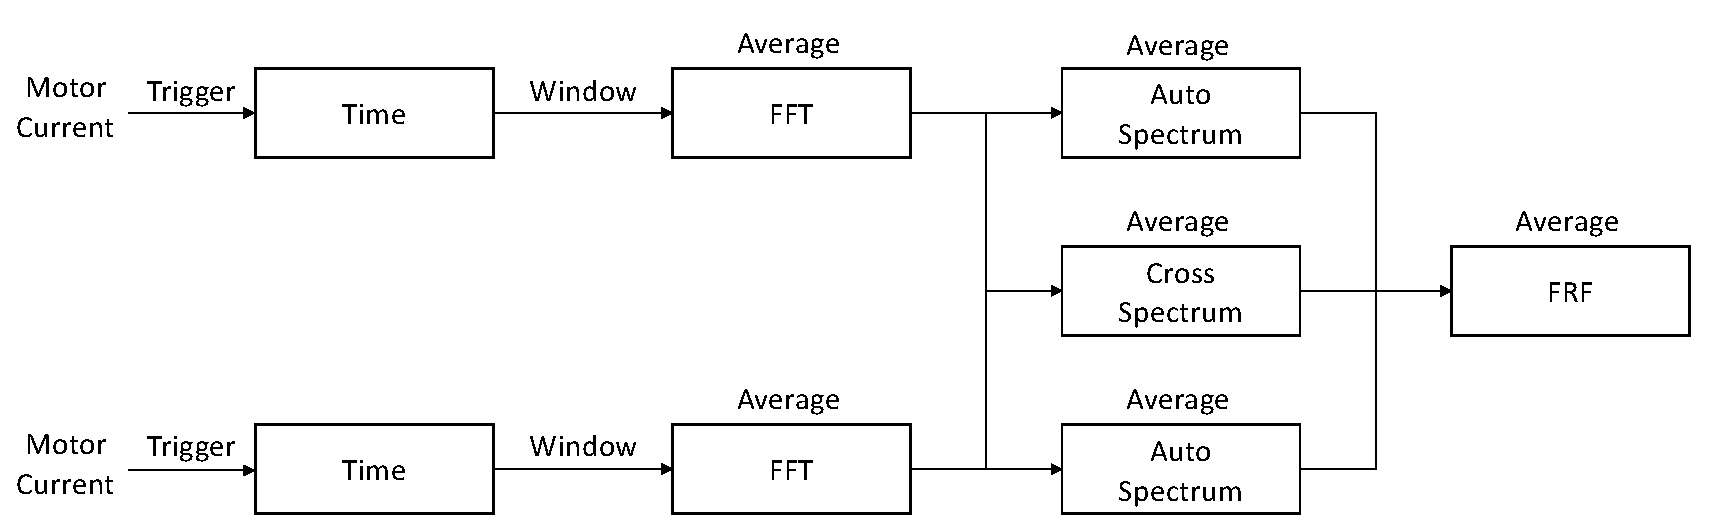
\includegraphics[width=.8\textwidth]{models_state_of_the_art/Nguyen_FRF.pdf}
  \caption{Average FRF calculation \cite{NGUYEN2019}}
  \label{fig:Nguyen_frf}
\end{figure}

\subsubsection{Conclusion}
Nguyen et al. \cite{NGUYEN2019} developed a complex inspection procedure to predict the preload of BSDs. The discrete dynamic model presented in fig. \ref{fig:Nguyen_discrete_dynamic_model} is the base of the preload prediction. The BSD system was simplified by springs and dampers. The quality of such prediction systems highly depends on the accuracy of the underlying model and its closeness to the real-world BSD. The modes of the BSD system were activated in extreme cases, where the motor changed its velocity rapidly. Only in these cases, the modes of the BSD were dominant enough to become visible and distinguishable from those of other components. The proposed BSD diagnosis was evaluated in a very supervised and isolated testbed. When inspecting BSDs installed in big industrial machines, the extraction of the axial natural frequency might become more challenging. The vibration from several other components might disturb the estimation of the modes of BSDs even more. The goal of such monitoring systems is the continuous estimation of the preload of BSDs over long time horizons. Operational conditions of industrial machines might not stay constant throughout those time horizons. In such cases, the established relationship between the axial natural frequency, the displacement of the working table and the preload of BSDs might not be reliable anymore. Even in the proposed isolated BSD testbed, the trigger sometimes failed to detect expressive operational phases for estimating the axial natural frequency. Implementing such a trigger for the BSDs in big industrial machines might be even more difficult. Nguyen et al. \cite{NGUYEN2019} emphasized that at least 10 trigger events from each position along the BSD screw shaft are required to average the FRF in practical applications properly. Collecting this big amount of trigger events involves a lot of effort and time. Equally to the work of Lee et al. \cite{Lee2015}, the BSD nut was used to record the vibration signal. It was not evaluated whether the axial natural frequency could be extracted from vibrations signals, recorded by sensors mounted in less fault-critical sensor locations. In the experiments, the preload the BSDs was changed by a built-in preload adjustment mechanism. The physical degradation of the shaft and the ball surfaces was neglected in the experiments.

\subsection{Data-Driven Approach: Sensor Fusion of Multiple Hand-Crafted Statistical Features}

Denkena et al. \cite{Denkena2021} presented a method to monitor the preload of BSDs. Firstly, several hand-crafted statistical features were extracted from the machine signals. Afterward, each feature was rated based on its robustness and statistical significance. The most promising signals were selected and fused based on the principal component analysis (PCA). At the end, decision trees solved the classification task. A testbed, consisting of a single BSD and linear guideways, was used to evaluate the proposed approach. The preload loss was simulated by installing ball sets with different oversizes. The internal controller provided internal control signals and three uniaxial acceleration sensors measured the system vibration. The machine data was recorded during a constant feed rate over the whole length of the test bench. The proposed PHM method can be separated into four steps:

\begin{itemize}
    \item [\textbf{Data acquisition:}] Signals from three uniaxial acceleration sensors and internal control signals were processed simultaneously. The signals were separated into phases of zero acceleration (constant movement of BSD nut on the BSD screw shaft) and non-zero acceleration (direction change movement of the BSD nut at each end of the BSD screw shaft). In the experiments, the ball screw was moved over the whole length of the test bench with various feed rates (6000 mm/min, 11000 mm/min, 17000 mm/min, 20000 mm/min) \cite{Denkena2021}.
    \item [\textbf{Feature extraction:}] Information about the preload classes were extracted through statistical features (e.g. kurtosis, median, impulse factor, ...). The features were applied to each signal and segment. At this point, the features were unrated. Each feature was evaluated by its robustness and statistical significance. The robustness was measured by the feature's dispersion around the median. After normalizing the feature with the z-score, the significance was estimated by the f-statistics.
    
    \begin{equation}
        \textbf{Z-score:}\qquad \tilde{x}_{i,j} = \frac{x_{i,j} - \bar x_{i}}{\sigma_{i}},
    \end{equation}
    
    \begin{equation}
        \textbf{F-statistic:}\qquad f = \frac{\sum_{j=1}^{J} i \cdot (\bar x_{j} -\bar x)^{2}/(J-1)}{\sum_{j=1}^{J} \sum_{i=1}^{I} i \cdot (\bar x_{j,i} -\bar x_{j})^{2}/(J \cdot (I-1))},
    \end{equation}
    where ${x}_{i,j}$ denotes the feature value j of a sample of class i, $\bar{x}_{i}$ is the feature mean value of class i, ${s}_{i}$ is the feature standard deviation of class i and $\bar{x}$ is the overall feature and class mean value, I and J are the number of all classes and features. Features were seen as eligible for the diagnosing system if the dispersion around the median was smaller than $\pm$ 10 and the f-statistic was higher than a critical value of 10 \cite{Denkena2021}. 
    
    \item [\textbf{Principal Component Analysis:}] 
    PCA is a method to reduce the dimension of data while retaining most of the information. Principal components are the directions in the feature space, along which the variation of the data is maximal. By using only a few principal components, each sample can be represented by a small number of variables \cite{Ringner2008}. By applying PCA, the selected features were merged with the goal of maintaining the robustness and increasing the f-statistics \cite{Denkena2021}.
    
    \item [\textbf{Classification:}] Decision trees were used to predict a preload class based on the extracted features. Due to its low classification effort and good traceability, decision trees are suitable for that classification task. For each signal and segment, a separate decision tree was used \cite{Denkena2021}. 
\end{itemize}

\subsubsection{Conclusion}
In order to find features that work well for predicting the BSD's degradation status, Denkena et al. \cite{Denkena2021} extracted 1500 features from the signal segments. For feed rates higher than 11000 mm/min, the acceleration signals were unsuitable for accurately predicting the preload classes. Some univariate features, like MAX, RMS and CRE, were only able to separate some of the defined preload classes. The robustness and statistical significance depended on the signals for some extracted statistical features. This shows that the suitability of the features generally depends strongly on the machine's working conditions, classes and signals.
Its limited robustness makes the application of the developed approach challenging for real-world tasks on industrial machines. The features did not show a proportional behavior to the physical degradation. When the features MAX and RMS were applied to the acceleration signals, they increased from C3 through C2 to C1, but decreased towards C0. Often deep learning is criticized for its black box principle and the lack of understanding of the extracted features. Even though one generally understands the hand-crafted features, the meaningfulness of the extracted information strongly depends on the task and signal. The correlation between those features and the physical degradation is often highly unknown, which makes such features an equal black box to features extracted by deep learning models. Dekena et al. \cite{Denkena2021} mentioned that slower feed rates improved the classification performance of some features. However, one has to consider that those slow feed rates also increase inspection time. Generally, one can say that finding a set of features that reliably predict all BSD preload classes demands substantial effort. These features work reliably for specific signals, working conditions and preload classes. If any of those specifications change, 
the entire system must be reconfigured completely. The physical degradation of the shaft and ball surface was neglected in the experiments.

\subsection{Data-Driven Approach: Multi-Level Feature Selection of Multiple Hand-Crafted Statistical Features}
Li et al. \cite{LiPin2018} developed a prognosis system for BSDs, which simultaneously performs fault diagnosis, early diagnosis, health assessment and remaining useful life (RUL) prediction. Since this thesis focuses on the fault diagnosis of BSDs, this chapter is restricted to the processing units related to diagnosis. A testbed was built containing a BSD and horizontal guideways fixed to a concrete base. Instead of manually inserting faults to simulate degradation, it was caused by field use. Fig.  \ref{fig:level_feature_selection_model} shows the different processing steps and the parallel prediction units for the fault diagnosis, health assessment and remaining useful life (RUL) prediction. Vibration data was recorded by three accelerometers and speed and torque signals were retrieved from the controller \cite{LiPin2018}. 

\begin{figure}[H]
  \centering
  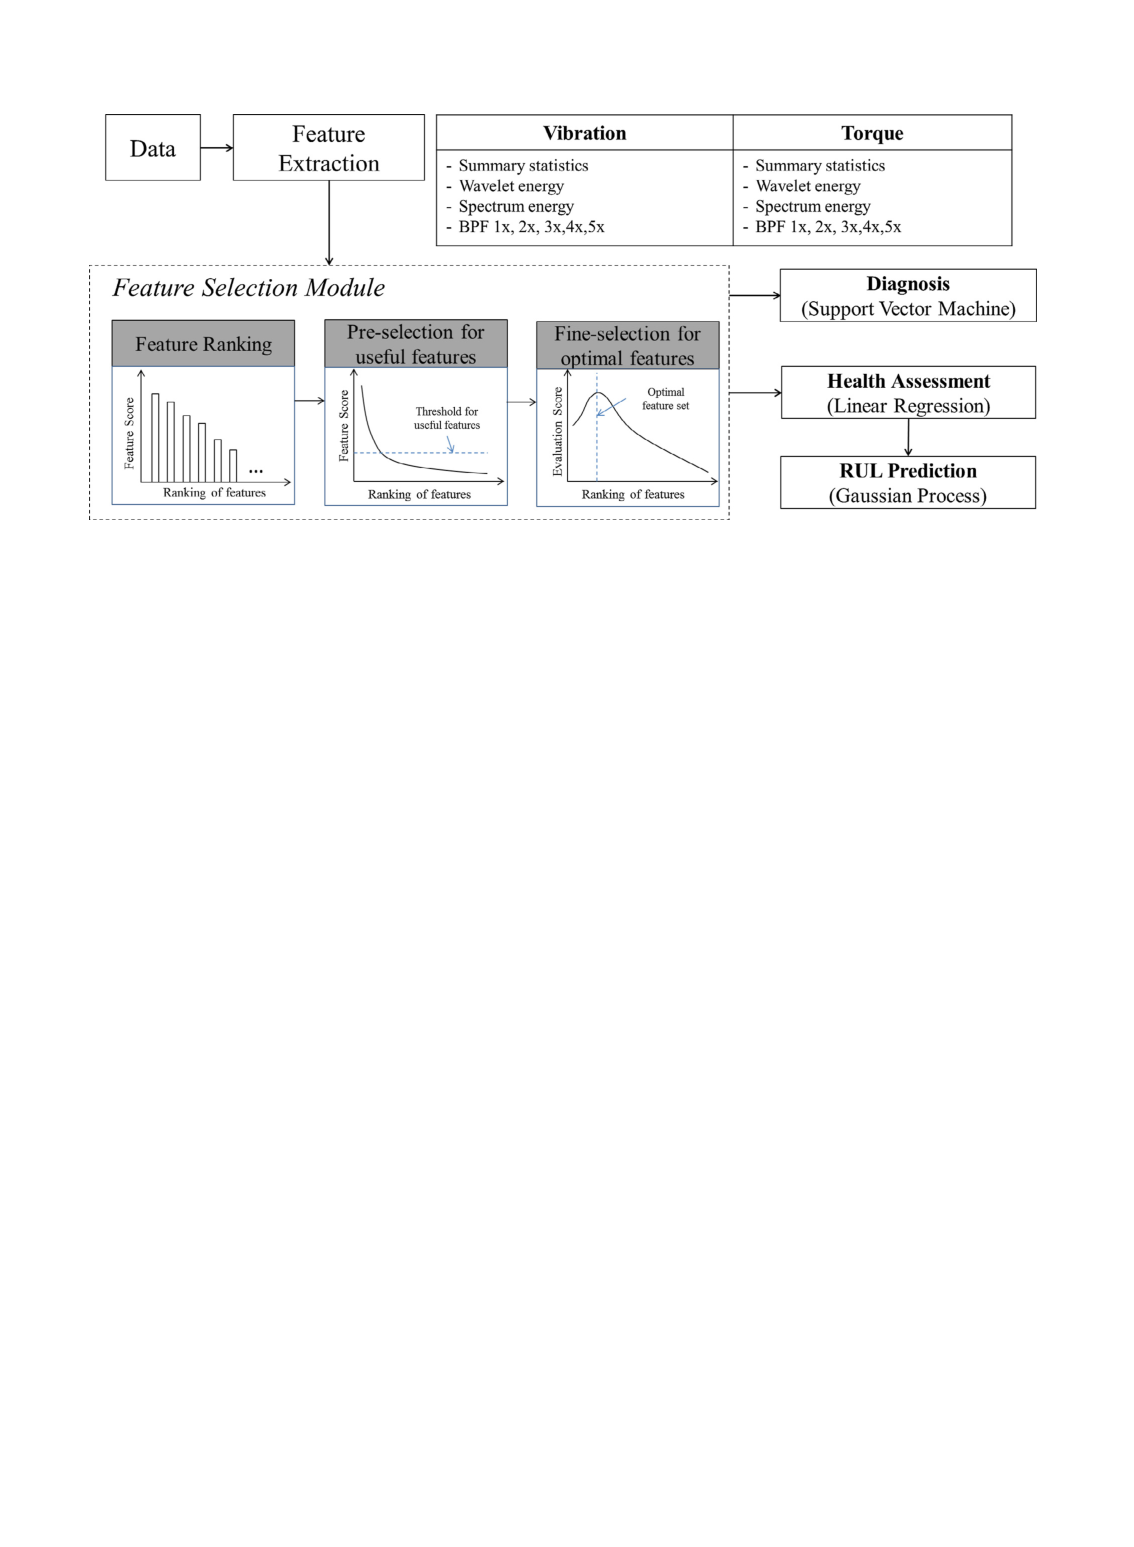
\includegraphics[width=1\textwidth]{models_state_of_the_art/model_multi-level_feature_selection.pdf}
  \caption{Feauture extraction and selection for health diagnosis, health assessment and RUL prediction \cite{LiPin2018}}
  \label{fig:level_feature_selection_model}
\end{figure}

In the following, the three diagnosis steps of the proposed PHM system are presented in more detail:

\begin{itemize}
    \item [\textbf{Feature Extraction}]: The system processed the signals in the time domain, frequency domain and time-frequency domain. The wavelet decomposition (‘db4’ wavelet) was applied to transform the signals. Similarly to Denkena et al. \cite{Denkena2021}, summary statistics, such as RMS, mean, variance, kurtosis and skewness, were extracted from the signals in all three domains (time domain, frequency domain and time-frequency domain). Like in the work of Lee et al. \cite{Lee2015}, the amplitudes corresponding to the calculated ball passing frequency and the ball screw rotation frequency, including its harmonics, were extracted as features for the monitoring system \cite{LiPin2018}.
    \item [\textbf{Feature Selection}]: In a multi-level feature selection procedure, the extracted features were rated by their suitability for the prognosis task. This process was separated into three stages: primary feature ranking, pre-selection and fine-selection. In order to select expressive features, a hybrid strategy of filter- (feature ranking and pre-selection) and the wrapper-based (fine-selection) approaches were applied. Wrapper methods rate features based on the performance of a classifier and filter-based methods pick features based on their intrinsic properties. In a multi-layer feature selection procedure, the search space and search sequence correspond to the features and their corresponding ranking scores found in the previous feature refinement phase. In the primary feature ranking phase, a selection criterion ranked and filtered all extracted features. In the pre-selection phase, the fisher score was applied to refine the previous feature choice:
    \begin{equation}
        S_{c} = \frac{\sum_{k=1}^{C} n_{k}(\mu_{k}^{j}-\mu^{j})^{2}}{\sum_{k=1}^{C}n_{k}(\sigma_{k}^{j})^{2}},
    \end{equation}
    where $C$ defines the number of classes, $n_{k}$ the number of samples in k-th class, $\mu_{k}^{j}$ and $\sigma_{k}^{j}$ the mean and standard deviation of the k-th class and the j-th feature and $\mu^{j}$ the mean of the j-th feature across all classes. For the multi-class classification task, the fisher score is biased. Therefore a fine feature-selection phase was added subsequently. Based on the prediction accuracy of an SVM, the final optimal features were selected \cite{LiPin2018}.
    \item [\textbf{Classification}]: A second SVM was applied to make the predictions for the diagnosis task. The SVM processed the optimal features found during the fine-selection phase \cite{LiPin2018}. 
\end{itemize}

\subsubsection{Conclusion}
From the raw data, Li et al. \cite{LiPin2018} extracted 440 features. In addition, three levels of feature selection and corresponding empirical thresholds were defined. For the vibration signals, the expressiveness of the different features varied a lot. The performance of some features diverged strongly when being applied to the vibration and torque signals. Similarly to the work of Denkena et al. \cite{Denkena2021}, some features did not correlate well with the degradation process. The definition of the empirical thresholds and application order of the different feature selection mechanisms was quite challenging. In the multi-level feature selection, the SVM-based fine-selection and fisher score-based pre-selection diverged in their feature ranking. Especially the top features found during the pre-selection were strongly downrated in the fine-selection. Defining the application order and therefore the significance of the different feature selection mechanisms strongly influenced the final feature choice. For the nine-class classification task, finding an empirical threshold for the fisher criterion was more challenging than for the binary classification task. All design choices for the feature extraction and selection are very specific and depend highly on the working conditions, health condition classes and signals. Minor variations in the predefined task specifications will most certainly reduce the system performance or make it even fail. Finding suitable feature extraction and selection mechanisms requires a huge effort. Using SVMs in the feature selection increases the training effort. This raises the training time and data requirements. Similarly to Nguyen et al. \cite{NGUYEN2019}, the physical degradation of surfaces in the BSD system was ignored. 


\section{Domain Adaptation Approaches for Prognostic and Health Management} \label{sec:domain_adaption_approach}
With the goal of developing robust monitoring systems for complex machines, adaptability and intelligence recently became more relevant for PHM systems. Inspired by the advances in the computer vision community, approaches from the area of domain adaptation and transfer learning achieve greater interest for industrial PHM. 

\subsection{Domain Adaptation Approaches for Prognostic and Health Management of Ball Screw Feed Drives}
In the following, deep learning-based domain adaptation models for monitoring the health condition status of BSDs are presented. Similarly to the method proposed in this thesis, the presented models apply the MMD to reduce the domain discrepancy.


\subsubsection{Deep Learning-Based Domain Adaptation Based on MMD-Loss}
Azamfar et al. \cite{AZAMFAR2020103932} proposed a deep learning-based domain adaptation model for estimating the health condition of BSDs based on their preload level. The preload was considered a good indicator for estimating the health condition of the BSDs and guideways. The domain discrepancy between the training and testing dataset was reduced by an MMD-loss. An experimental test rig was built, containing a single horizontal guideway and a BSD fixed on a concrete base. Three accelerometers were installed to measure vibrations in X and Y directions. These sensors were mounted on the BSD nut and the bottom and top attachments of the BSD screw shaft. A sound pressure sensor captured the acoustic level during the experiments on the test rig. The torque and speed signals were acquired from the controller. Three different preload classes were defined for the guideways and BSDs. In the "normal" class the component is operating normally, in the "faulty level 1" class it is deviating from the healthy condition and in the "faulty level 2" class it needs to be replaced or repaired. In total, nine combinations of guideway and BSD degradation classes were defined. Data was recorded by performing a full cycle of BSD operation, containing two full forward and backward movements along the guideways. The signals were split in phases of constant and changing BSD nut velocity. The training was restricted to those segments with constant BSD velocity, which were fed to the model as single samples. The data dimension was reduced by a simple down-sampling method. The recordings included BSD operations with different BSD velocities (200, 400 and 600 mm/s). Recording the data with different BSD velocities created a domain shift between the training and testing dataset. The proposed method was evaluated on the nine-class classification task, including all combinations of BSD and guideway degradation classes. The proposed neural network architecture is presented in fig. \ref{fig:Azamfar_model}. It contained a CNN of four alternating 1D convolutional and max-pooling layers and a subsequent classifier. To prevent overfitting, dropout layers with a rate of 0.3 were included. ReLU activation functions were used throughout the network. The proposed model optimization included a source CE-loss to improve the classification accuracy on the source domain data. Besides that, the domain discrepancy was reduced by an MMD-loss, which was applied in the penultimate fully connected layer. 

\begin{figure}[H]
  \centering
  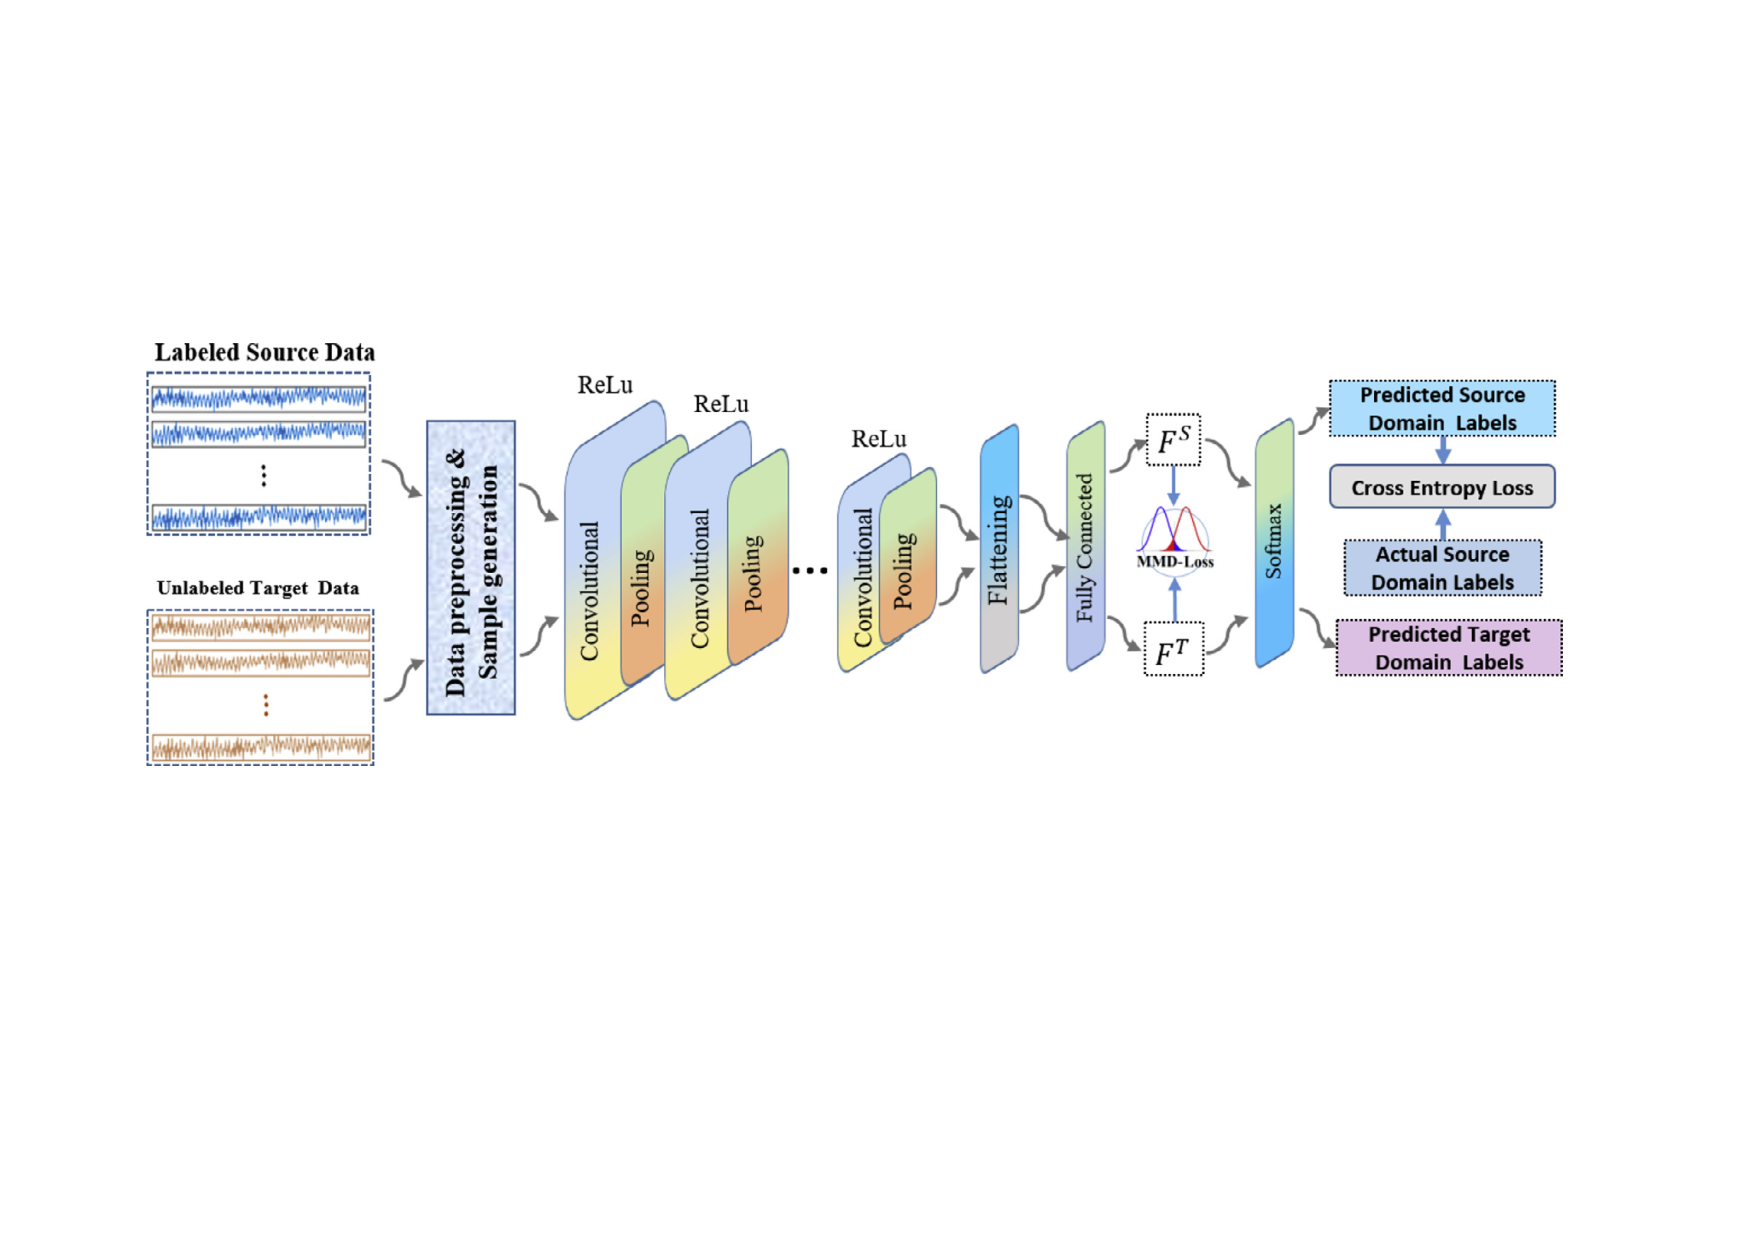
\includegraphics[width=1\textwidth]{models_state_of_the_art/Azamfar_model.pdf}
  \caption{Model architecture of deep learning-based domain adaptation model for PHM of BSDs using an MMD-loss \cite{AZAMFAR2020103932}}
  \label{fig:Azamfar_model}
\end{figure}


\subsubsection{Deep Learning-Based Domain Adaptation Based on MMD-Loss and PD Alignment}
Similarly to Azamfar et al. \cite{AZAMFAR2020103932}, Pandhare et al. \cite{Pandhare2021} proposed a deep learning-based domain adaptation model for estimating the health condition of BSDs based on their preload level. The domain discrepancy between the training and testing dataset was reduced by an MMD-loss and PD alignment. A similar test rig, as the one presented by Azamfar et al. \cite{AZAMFAR2020103932}, was used to evaluate the proposed models. In total, five accelerometers were mounted on the testbed. Two triaxial ones were placed close to the BSD nut, which is a promising position to represent the signature of the ball screw preload level. Three single-axial ones were mounted at the bottom and top attachments of the BSD screw shaft and on top of the load carried by the BSD nut. These sensor positions are more suitable and practical installations. Identical to Azamfar et al. \cite{AZAMFAR2020103932}, nine combinations of BSD and guideway preload classes were defined. By recording data with sensors mounted at different positions in the BSD testbed, a domain shift was created. Pandhare et al. \cite{Pandhare2021} tried to find an indirect sensing method to make PHM independent of impractical sensor locations. The proposed model architecture is presented in fig. \ref{fig:Pandhare_model}. It contained a CNN of two alternating 1D convolutional and max pooling layers and a consecutive classifier. The proposed model training included three losses. Again, a source CE-loss was used to improve the classification performance on the source domain data. The MMD loss reduced the marginal and the PD alignment the conditional distribution discrepancy between the domains. The PD alignment matched source and target samples of the same class and reduced their L2-distance: 

\begin{equation}
    L_{p} = \frac{1}{n_{p}}\sum_{k=1}^{n_{p}}|h_{k}^{p,s}-h_{k}^{p,t}|_{2}, 
\end{equation}
where $h_{k}^{p,s}$ and $h_{k}^{p,t}$ are the k-th source and target domain samples and $n_{p}$ is subspace of the labeled samples from source and target. The PDalignment was restricted to some of the nine classes and 20\% of the training samples were used as PD samples.
\begin{figure}[H]
  \centering
  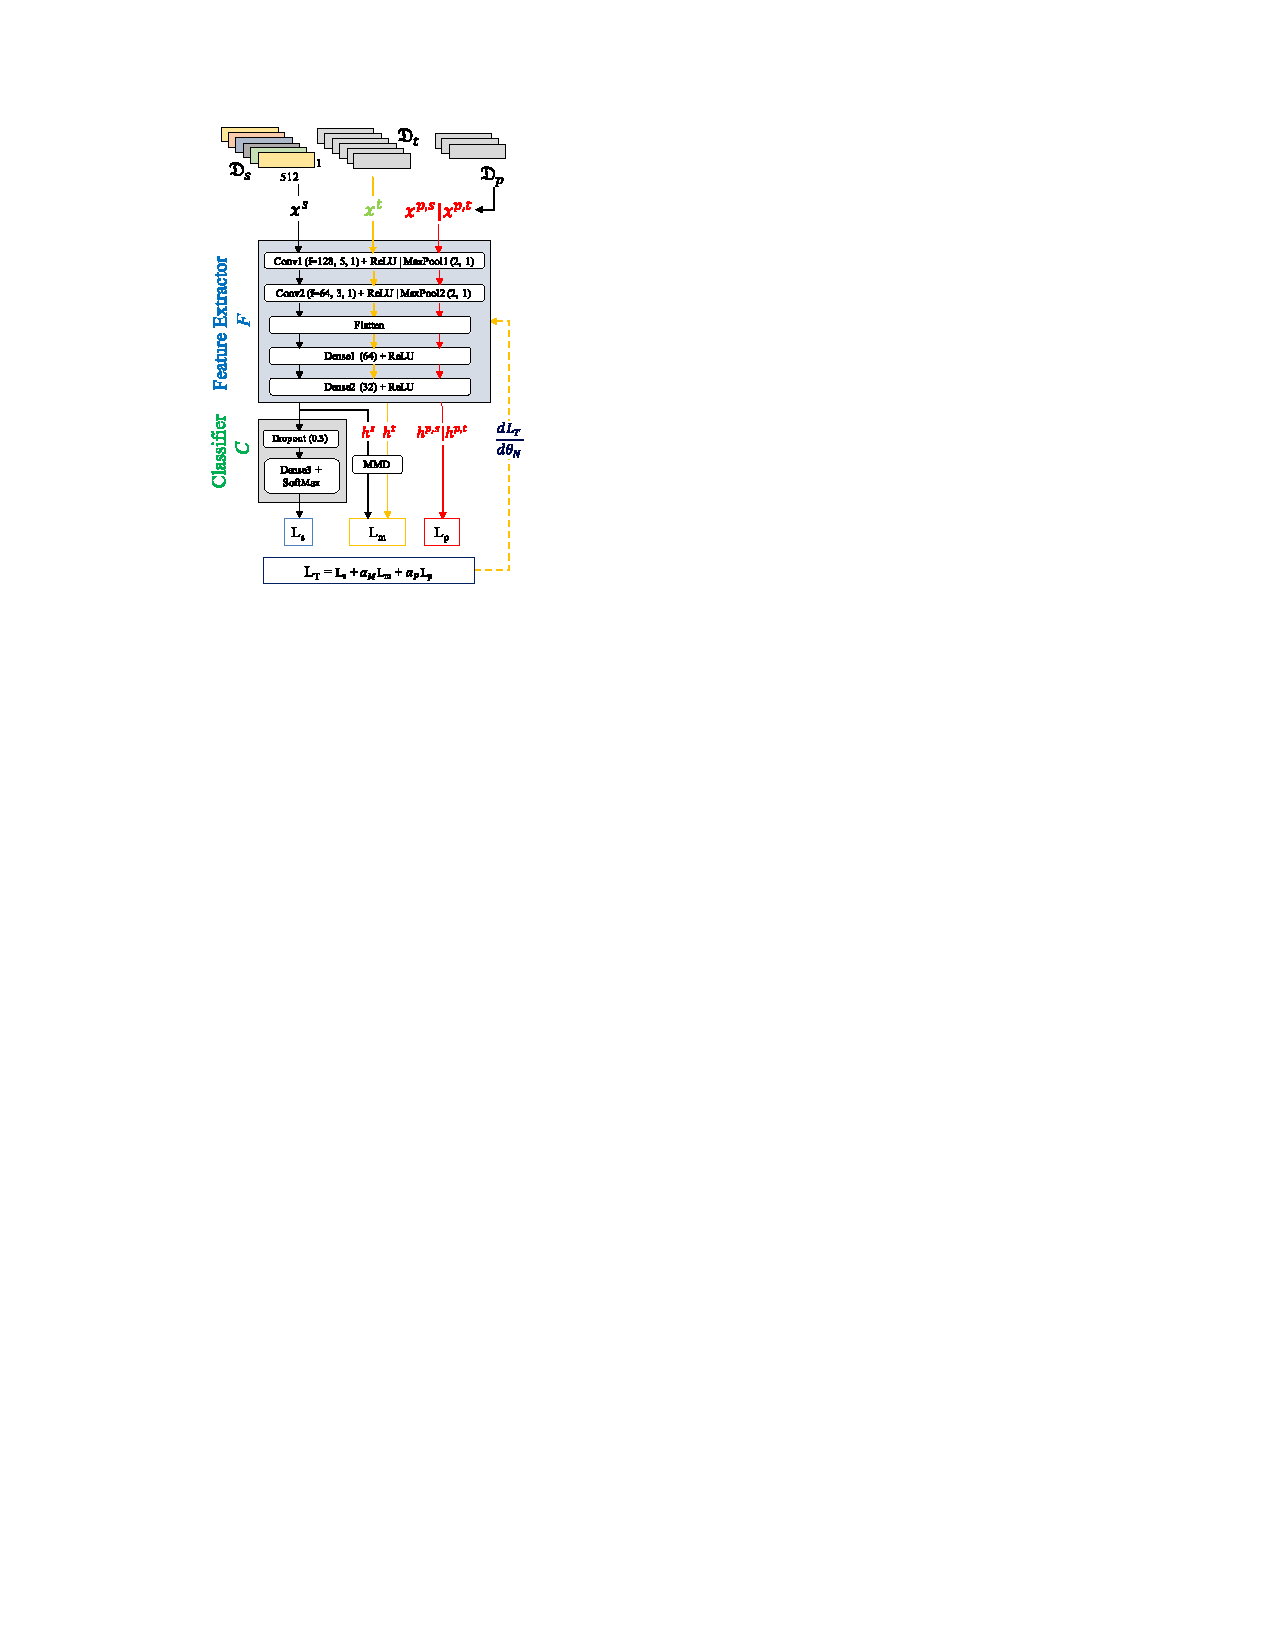
\includegraphics[width=.6\textwidth]{models_state_of_the_art/Pandhare_model.pdf}
  \caption{Model architecture of deep learning-based domain adaptation model for PHM of BSDs using an MMD-loss and PD alignment \cite{Pandhare2021}}
  \label{fig:Pandhare_model}
\end{figure}

\subsubsection{Conclusion}
The similar problems and disadvantages of the presented approaches by Azamfar et al. \cite{AZAMFAR2020103932} and Pandhare et al. \cite{Pandhare2021} are collectively presented in this section. First of all, both approaches applied a regime separation to split the signals into phases of constant and changing BSD velocity. This extra step adds additional complexity to the data pre-processing. Both approaches did not window the signals. The segments with constant BSD velocity were fed to the models as single samples. Since those samples capture the frequency and amplitude variations during the whole steady-state phase of the BSD operation, they were assumed to be more informative for the monitoring task. By doing so, only a few samples were collected from the recordings of each experiment. A lot of experimental effort is required to record enough samples to train the neural network properly. Azamfar et al. \cite{AZAMFAR2020103932} and  Pandhare et al. \cite{Pandhare2021} evaluated their monitoring approaches solely on a simplified testbed. Therefore, the evaluation of the approaches did not consider the mutual influence of other components installed in real industrial machines. Besides that, both approaches were restricted to predicting BSD preload forces. Other damages, like pitting, were ignored by the monitoring systems. In both cases, the MMD-loss was solely applied in the last fully connected layer. The domain discrepancy reduction was not evaluated in any other latent feature map of the model. Azamfar et al. \cite{AZAMFAR2020103932} created a domain shift by recording data with different BSD velocities and Pandhare et al. \cite{Pandhare2021} by recording data with accelerometers mounted at different positions in the BSD testbed. In both cases, the domain shift was not generated by any differences on the physical component level. The same components were represented in both domains and therefore also in the training and testing dataset. The PHM systems did only have to deal with domain shifts created by variations in the BSD operational conditions and data recording. It was not evaluated how the presented approaches react to physical variations in the systems. The PD alignment approach, presented by Pandhare et al. \cite{Pandhare2021}, requires target labels from some of the considered classes. This simplifies the health condition monitoring task and is impractical for real-world PHM systems.

\subsection{Domain Adaptation Approaches for Prognostic and Health Management of Rolling Bearings}

A PHM algorithm for rolling bearings, which optimizes the inter- and intra-class distance in the latent feature space and reduces the domain discrepancy with an MMD-loss, was presented by Li et al. \cite{Li2018}. As visualized in fig. \ref{fig:Deep_distance_metric_learning_model}, the proposed model contained a CNN and a consecutive classifier. In a preprocessing step, a FFT transform was applied to represent the raw vibration signals in the time-frequency domain. Max-pooling layers were included to reduce the model size. Batch-normalization layers reduced the internal covariate shift by normalizing the input distributions of the hidden layers. To prevent overfitting, dropout layers with a rate of 0.5 were included. The proposed method was evaluated on a rolling bearing dataset provided by the Bearing Data Center of Case Western Reserve University. The domain shift was generated by using testing data, which was exposed to additional environmental noise and collected under different working conditions. Ten health conditions with faults in different locations and with varying extents were defined. 

\begin{figure}[H]
  \centering
  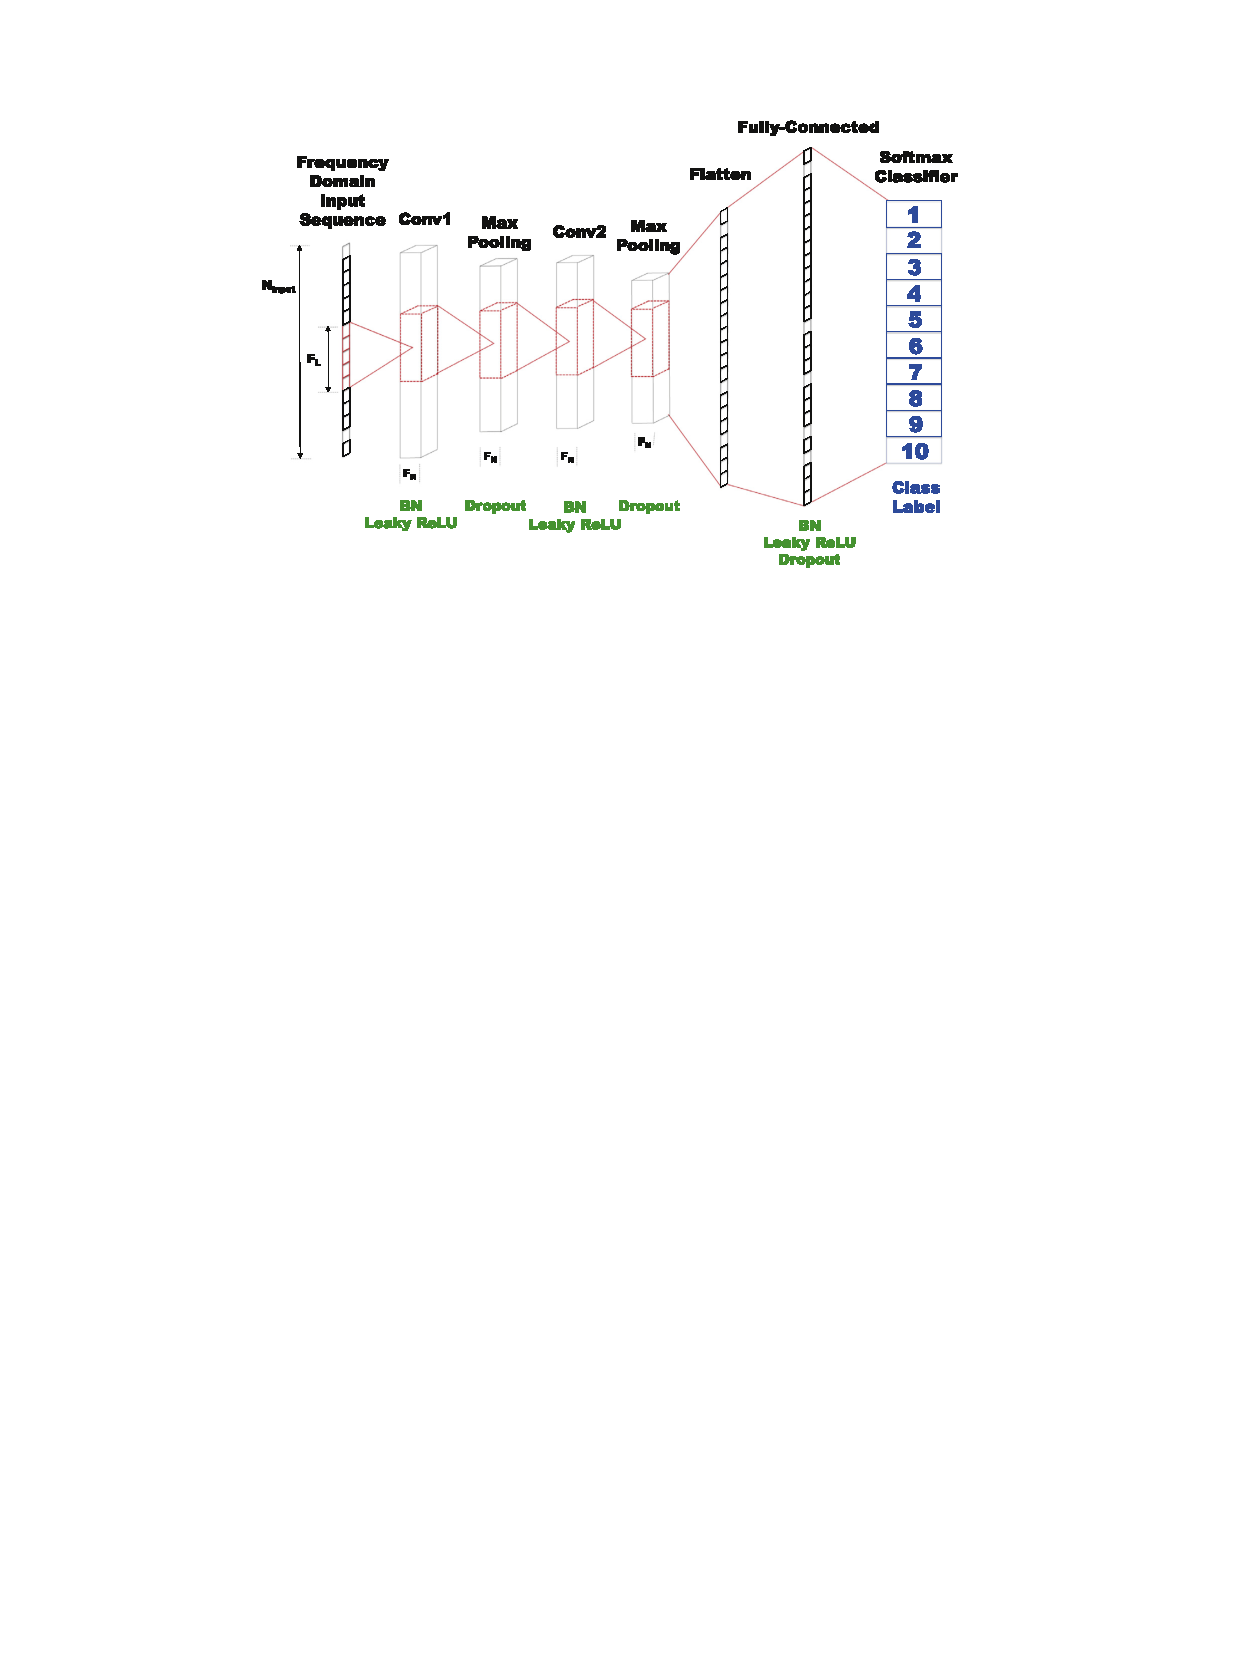
\includegraphics[width=.75\textwidth]{models_state_of_the_art/Deep_distance_metric_learning_model.pdf}
  \caption{Model architecture of deep learning-based domain adaptation model for PHM of rolling bearings using deep distance metric learning \cite{Li2018}}
  \label{fig:Deep_distance_metric_learning_model}
\end{figure}

The distance between the source samples was minimized if they did belong to the same class and maximized otherwise. This increased the separability and compactness of the source domain classes, which makes the algorithm more robust against environmental noise. In order to calculate the intra- and inter-class distances, the expectation and variance of the source domain samples belonging to the same class were measured in the feature maps:

\begin{equation}
    \begin{aligned}
       &D_{inter} = |E[f^{(m)}x^{(i)}]-E[f^{(m)}x^{(j)}]|_{2}-\sqrt{Var[f^{(m)}x^{(i)}]}-\sqrt{Var[f^{(m)}x^{(j)}]}\\
       &D_{intra} = 
        \sum_{i=1}^{N_{class}} \sqrt{Var[x^{(i)}]},
    \end{aligned}
\end{equation}

where $N_{class}$ is the number of classes, $x^{(k)}$ denotes the raw input sample of class k, $f^{(m)}x^{(k)}$ denotes the feature representation of this sample in the m-th layer and $E[f^{(m)}x^{(i)}]$ and $Var[f^{(m)}x^{(i)}]$ are the corresponding expectation and variance. The inter- and intra-class distance were optimized with the following loss: $J_{Cluster} = - D_{inter} + \eta D_{intra}$. In addition to the distance metric learning, the discrepancy between the source and target domain was reduced by an MMD-loss applied in several FC layers. Lastly, the CE-loss in the final layer optimized the model to classify the source samples correctly. In total, the network was trained with the following weighted average of losses: 

\begin{equation}
    \begin{aligned}
    J_{total} = \alpha J_{Cluster} + \beta J_{MMD} + \gamma J_{CE}, 
    \end{aligned}
\end{equation}
where $J_{Cluster}$ is the loss, optimizing the distances between the source domain samples, $J_{MMD}$ the MMD-loss,  $J_{CE}$ the CE-loss and $\alpha$, $\beta$ and $\gamma$ are the weights for calculating the weighted average \cite{Li2018}.

\subsubsection{Conclusion}
There are several MMD-based domain adaptation approaches for PHM of rolling bearing \cite{AN201942} \cite{Li2018} \cite{Guo2019} \cite{Singh2019} \cite{Kang2020}. Generally, BSDs and rolling bearings are related components. BSD screw shafts can be seen as the inner and BSD nuts as the outer ring of rolling bearings \cite{Lee2015}. In both cases, balls between those two components allow a rotatory motion around a fixed axis. Besides rolling bearings, BSDs also translate this rotatory motion into a linear one. The degradation of rolling bearings and BSDs is related in some sense. However, bearing PHM applications cannot be relied on to work as well for BSDs. Still, the research in this domain offers interesting applications and details for the PHM of BSDs. 

\section{CNN-Based Domain Adaptation in Computer Vision Applications} \label{sec:domain_adaption_CV}

\begin{comment}
\subsection{Domain Conditioned Adaptation Network}
Li et al. \cite{li2020} propose a domain conditioned adaptation network (DCAN), which contains two separate modules to reduce the domain discrepancy. After each task-specific layer a domain conditioned feature correction block estimates and reduces the domain discrepancy based on the MMD metric. In the CNN backbone an attention module regulates the extraction of domain-specific and -independent features. The proportions of domain-specific and -independent features is learned to decrease the domain discrepancy. Fig. \ref{fig:DCAN_model} visualizes the domain adaptation modules in the DCAN model.

\subsubsection{Domain Conditioned Channel Attention Mechanism}
ResNet is used as a backbone network, which allows an easy implementation of the domain conditioned channel attention module in its residual block. In the latent feature maps, the processed images are represented as $\pmb{X}_{t} = [X^{1}_{t},...,X^{C}_{t}] \in \mathbb{R}^{HxWxC}$, where H and W are the spatial dimension and C the number of image channels. First, a channel-wise global average pooling layer is applied, which reduces the images to  $\pmb{g}_{t} = [g^{1}_{t},...,g^{C}_{t}] \in \mathbb{R}^{1x1xC}$. Afterwards, the data is split depending on its domain and passed through different fully connected layers. The upper flow is used for target and the lower flow for source domain samples. The two different source and target domain routes share parameters. For both domains, an attention mechanism is trained jointly to learn activating different channels in the domain samples. This allows extracting more enriched domain-specific features. In the fully connected layers the dimension is first reduced with a ratio ${1x1x\frac{C}{r}}$ and later reconstructed to its original size ${1x1xC}$. ReLU and Sigmoid functions are applied. The domain-wise feature selection is achieved by weighting the channels of the feature representations $\pmb{X}_{s}$ and $\pmb{X}_{t}$ with the channel attention vectors $\pmb{v}_{s}$ and $\pmb{v}_{t}$ calculated by the domain conditioned channel attention module:

\begin{equation}
    \begin{aligned}
        &\pmb{\tilde{X}}_{s} = \pmb{v}_{s} \odot \pmb{X}_{s} = [v_{s}^{1} \cdot X_{s}^{1}, ..., v_{s}^{C} \cdot X_{s}^{C}]\\
        &\pmb{\tilde{X}}_{t} = \pmb{v}_{t} \odot \pmb{X}_{t} = [v_{t}^{1} \cdot X_{t}^{1}, ..., v_{t}^{C} \cdot X_{t}^{C}].
    \end{aligned}
\end{equation}

The domain conditioned channel attention module allows the model to independently learn the importance of each channel for the classification of source and target domain samples \cite{li2020}.

\subsubsection{Domain Conditioned Feature Correction}
The data simultaneously passes through the regular network and the feature correction block, which consist of FC and ReLU blocks. The feature correction block estimates the domain discrepancy in the feature representation of the task-specific layer:
\begin{equation}
    \Delta H_{l}(x_{t}) = H_{l}(x_{s}) - H_{l}(x_{t}),
\end{equation}
where $H_{l}(x_{s})$ and $H_{l}(x_{t})$ are the feature representations of the source and target domain samples in the task-specific layer l. $\pmb{x}_{s}$ and $\pmb{x}_{t}$ are the source and target domain samples. The feature representation of the target domain samples is corrected as following:

\begin{equation}
    \hat{H}_{l}(x_{t}) = H_{l}(x_{t}) + \Delta H_{l}(x_{t}).
\end{equation}

The discrepancy between the regular feature representation of source domain samples $H_{l}(x_{s})$ and the corrected feature representation of the target domain samples $\hat{H}_{l}(x_{t})$ is measured by the MMD-loss in several layers:

\begin{equation}
    L_{M}^{l} = |\frac{1}{n_s} \sum_{i=1}^{n_{s}} \phi(H_{l}(x_{si}) - \frac{1}{n_t} \sum_{i=1}^{n_{t}} \phi(\hat{H}_{l}(x_{ti}))|_{H_{\kappa}}^{2}, 
\end{equation}
where $H_{\kappa}$ is the reproducing kernel Hilbert space (RKHS), $\kappa$ the characteristic kernel and $\phi$ the corresponding feature map. The number of source and target samples is defined by $n_{s}$ and $n_{t}$. To avoid the over-transfer of noise and irrelevant information between source and target, the model is enforced to keep the source data constant when passing through the feature correction blocks \cite{li2020}.

\begin{figure}[H]
  \centering
  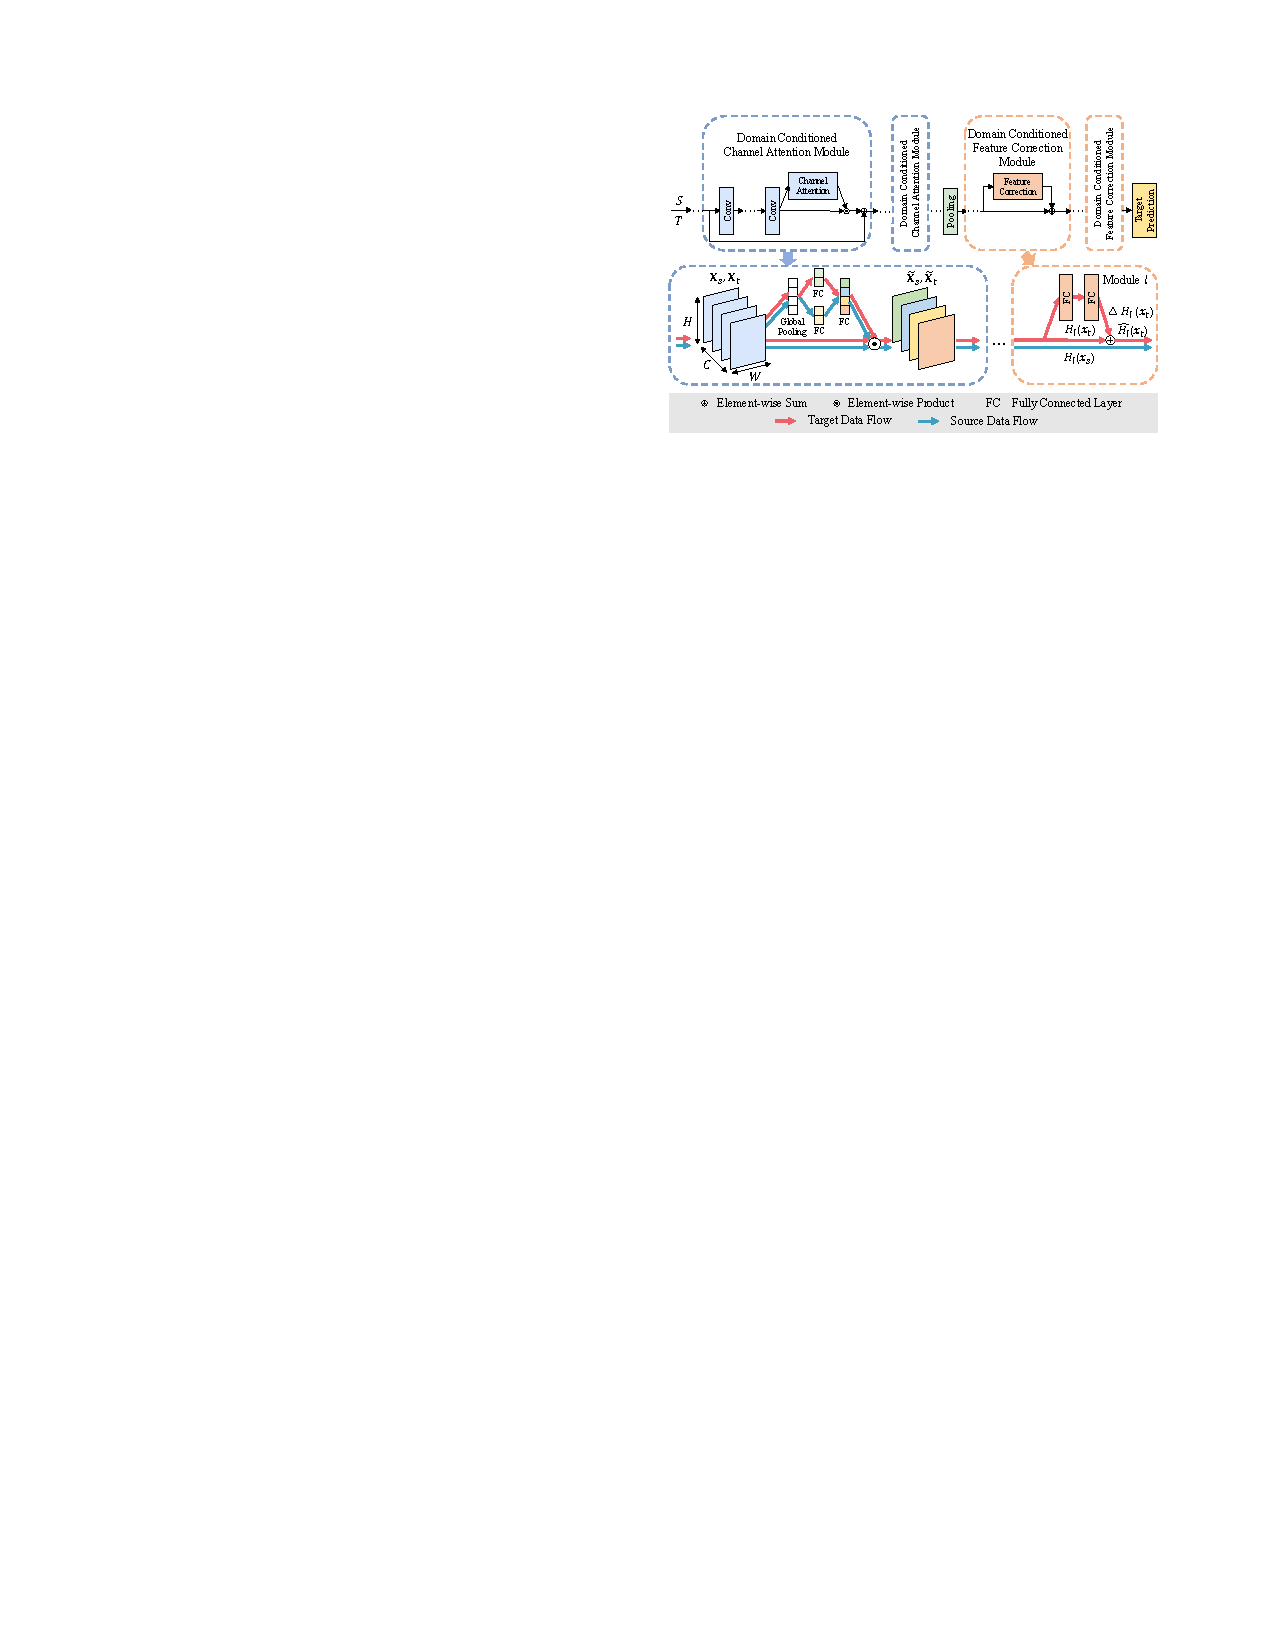
\includegraphics[width=1\textwidth]{models_state_of_the_art/DCAN_model.pdf}
  \caption{DCAN architecture proposed by Li et al. \cite{li2020}}
  \label{fig:DCAN_model}
\end{figure}

\end{comment}

%\subsection{Feature Reconstruction of Domain Shift Affected Layers}
Aljundi et al. \cite{Aljundi2016} presented a domain adaptation approach for computer vision applications. The method analyzed the domain shift effects in all convolutional layers of the neural network. Strongly affected feature maps (bad filters) were identified and reconstructed by less affected ones (good filters). During the optimization, one filter map was considered at a time. The goal was to identify those feature maps which were able to reconstruct the response of the evaluated one. The feature map was reconstructed by a weighted average of all feature maps. This kind of optimization simultaneously recognized bad feature maps and identified corresponding good ones for their reconstruction. Additionally, the optimization measured the domain discrepancy of the feature maps with the Kullback-Leibler (KL) divergence and punished the feature map's influence during the reconstruction process accordingly:  
\begin{equation}
    B^{*} = argmin_{B} \{ \sum_{i=1}^{n}( y_{i}-\beta_{0}-\sum_{j=1}^{p}x_{i,j}\beta_{j})^{2} + \lambda \sum_{j=1}^{p}|\Delta_{j}^{KL}\cdot \beta_{j}| \}
\end{equation}
where $y_{i}$ is the output of the evaluated filter map for the sample $i$, $x_{i,j}$ the output of the feature map $j$ for the sample $i$, $\beta_{0}$ the residual, $B = \{\beta_{j}\}$ the coefficients, estimating the suitability of each feature map to reconstruct the output of the evaluated feature map, $n$ the number of source samples, $p$ the number of layers, $\lambda$ a tuning parameter to punish the coefficients and $\Delta_{j}^{KL}$ the KL divergence measured between the source and target data representations in layer $j$. When a layer's coefficient  $\beta_{j}$ was big, it was considered as good (small domain shift effects) and otherwise as bad (big domain shift effects). The optimization was solved by using the coordinate descent method. In a second step, linear regression was applied to reconstruct the output of the bad layers by a weighted average of the good ones. The reconstructed layer outputs were then passed to the subsequent layers. Aljundi et al. \cite{Aljundi2016} identified the CNN's early layers to be especially relevant to counteract the domain shift.

\subsubsection{Conclusion}
The presented approach by Aljundi et al. \cite{Aljundi2016} disagrees with most domain adaptation approaches, which reduce the domain discrepancy in task-specific layers but use a shared CNN backbone across all domains. The work shows the positive effect of reducing the domain shift in the early layers of the CNN. Often there is no clear pattern of which layers contribute most to the domain discrepancy problem. Therefore, it is a great approach to evaluate each layer individually and adapt the domain reduction adequately. The work shows, that early layers in the CNN already suffer from and significantly contribute to the domain shift. Aljundi et al. \cite{Aljundi2016} gave a great hypothetical example of how early layers of CNNs can generate domain shifts. If one imagines a model for recognizing facial expressions, early layers of the CNN usually detect things like colors and edges. When training such a model with young faces and testing it with those of old people, the system would be confronted with wrinkles, which it would not have seen during training. These wrinkles could distract the system to recognize those edges, which are relevant for identifying facial expressions. By adapting those early layers, which are responsible for edge detection, to be less prone to wrinkles, the domain shift could be reduced efficiently \cite{Aljundi2016}. Often the computer vision community offers advanced solutions for complex research questions which were not intensively evaluated in real-world scenarios. For the PHM of BSDs such solutions can be taken as inspiration. 

\section{Research Gap}
When industrial machines run over long time horizons, variations in the operational conditions change their fault characteristics. Due to the mutual influence of the different machine's submodules, fault characteristics are often complex and highly dependent. Developing hand-crafted features, as they are quite common in traditional approaches, requires a lot of experience and human labor. Due to the lack of flexibility and robustness, hand-crafted features struggle to extract expressive information from the data when the corresponding fault characteristics vary over time. Model-based PHM systems, like those presented by Lee et al. \cite{Lee2015} and Nguyen et al. \cite{NGUYEN2019},  predict the BSD's health condition based on simplified physical models. The quality of those approaches highly depends on the exactness and sophistication of the underlying models and the corresponding parameters. If the models miss details from the real-world machines and the underlying processes, the PHM performance will be unsatisfactory. Data-driven PHM systems, like those proposed by Denkena et al. \cite{Denkena2021} and Li et al. \cite{LiPin2018}, use trainable classifiers in the final steps of the processing chain. These classifiers learn to use the information extracted by the hand-crafted features to make accurate predictions. This intelligent way of combining the retrieved knowledge from the data might make those systems less prone to minor variations in the fault characteristics. Since these models automatically learn the correlation between the machine data and health condition classes, adapting such systems to new circumstances is often less time-consuming. Nevertheless, the system's performance highly depends on the underlying training dataset. It is unlikely that the data used for training includes all operational conditions and fault scenarios. It can even happen that fault classes are unknown during training. Optimizing neural networks with limited data, which does not represent the data distributions during testing, might lead to a low diagnosis performance \cite{AZAMFAR2020103932}. Robust PHM systems, designed to handle fault characteristic changes reliably, would bring industrial PHM systems to the next level \cite{Michau2017}. In order to address these issues, PHM systems can be extended with domain adaptation modules. This thesis investigates the applicability and usability of deep learning-based domain adaptation for health condition monitoring of BSDs. The advantages of the proposed system over regular deep learning-based systems are evaluated. It requires a lot of work to establish accurate physical models and expressive hand-crafted features, which capture the degradation of BSDs. For this reason, the developed approach in this thesis is not compared to any traditional model-based or data-driven PHM system. Most MMD-based domain adaptation systems for PHM applications, like those presented by Pandhare et al. \cite{Pandhare2021} and Azamfar et al. \cite{AZAMFAR2020103932}, apply MMD-losses in task-specific layers. The literature rarely discusses variations in the MMD application, which could reduce the domain discrepancy more efficiently. Inspired by the computer vision community, this thesis evaluates different MMD-loss types and corresponding hyperparameters for monitoring the health condition of BSDs. The works presented by Pandhare et al. \cite{Pandhare2021} and Azamfar et al. \cite{AZAMFAR2020103932} evaluated their models on a simplified testbed. A dataset was recorded, which used the same physical BSD and LGS components in the training and testing dataset. In this thesis, the developed models were tested on data recorded on a real-world machine. Differences on the physical component level created the domain shift. Furthermore, the prediction of the BSD's health condition classes was tested with differently degraded LGSs. Compared to most works in the literature, the evaluation in this thesis is more realistic and the PHM task more challenging. 
